%\appendix
\chapter{Theoretical Performance Models}

\section*{Amdahl's Law}
\label{AmdahlsLaw}

The speedup that can be achieve by parallelizing an application is not only dependent on the number of parallel tasks but also on the percentage of the code that will run in parallel. This means that it is possible to have an extremely optimized implementation of the parallelization but if only a small part of the code is parallel the speedup will be small.

Amdahl's Law \cite{AMDAHL} defines the maximum attainable speedup of parallelizing an application, comparing a multithreaded application using $N$ processors with its serial counterpart. The law takes into account the portion of the code, $P$, that can be paralelized and defines the maximum speedup $S$ that can be obtained.

\begin{center}
	\begin{equation}
		S(N) = \frac{1}{(1 - P) + \frac{P}{N}}
		\label{eq:Amdahl}
	\end{equation}
\end{center}

Equation \ref{eq:Amdahl} defines the maximum attainable speedup resultant from the parallelization of an application according to the Amdahl's Law. The law is used in this work to prove that the small speedups for fewer number of variations per event are close to the theoretical maximum and are limited by the percentage of the code that can be made parallel.

\section*{Roofline Model}
\label{App:Roofline}

The Roofline model \cite{Roofline} was used characterize the system in terms of attainable peak performance. This model uses two metrics for the performance calculation, the peak CPU performance and the memory bandwidth. With the peak values of these two metrics a roofline is drawn, which is the theoretical limit for the system performance. Other ceilings can then be added, further limiting the reachable performance. The classic Roofline uses float point computation as the peak CPU performance metric, which is usually advertised as peak performance of the hardware by manufacturers. It may be a good metric for heavy computational algorithms, such as matrix algebra. The instruction mix presented in section \ref{ComputationalCharactrization} shows that the type operations on the critical region of \tth (the \ttDilepKinFit function) is much more varied than only floating point arithmetic. The computational intensity was used for measuring the CPU peak performance, as it considers all types of instructions.

The peak computational intensity is calculated with the formula \ref{eq:CompIntensity}. The clock frequency and number of cores are easily obtained by consulting the CPU specifications, while the number of instructions issued per clock cycle is more difficult to determine. It is based on the super scalarity degree of the processor, i.e., the number of instructions that can be decoded per clock cycle, and then it must be confirmed if the number of possible instructions issued match with the number of functional units. The value obtained makes the horizontal roof of the model. The tilted roof of the Roofline model refers to the maximum memory bandwidth of the system and it was determined using the stream benchmark. These values are presented in appendix \ref{App:TestEnv}.

\begin{center}
	\begin{equation}
		C = Clock Freq. * # of Cores * # of Instructions per Clock
		\label{eq:CompIntensity}
	\end{equation}
\end{center}

Further ceilings can be added, defining factors, at the hardware level, which may affect the performance. The most common ceilings are presented in the Roofline model for the test system are characterized below:

\begin{description}
	\item[One processor:] the usage of one CPU in a dual-socket system halves the maximum performance as only is used half of the available computational resources.
	\item[TLP:] thread level parallelism (TLP) allows exploiting the usage of all available cores in one CPU. If only one core is used, the maximum performance is limited by a factor equal to the number of cores.
	\item[Mul/Add balance:] each CPU core has two functional units, one for additions and other for multiplications and divisions. If an algorithm only has additions or multiplications, one of the functional units will be idle, halving the performance. The algorithm must have a approximate number of additions and multiplications to simultaneously use both functional units, and they must be intercaleted in such a way that the instruction dispatcher is able to keep both units always occupied.
	\item[ILP:] the performance will be highly affected if the instruction level parallelism is not used. Considering an addition as an example, which takes 2 clock cycles to compute, if only one instruction is issued every 2 cycles the performance is half of the performance if one instruction is issued every cycle. Considering other functional units, such as divisions that use many more clock cycles, the performance could be even more affected.
	\item[No Triple Channel:] the CPU on the compute-601 node has 3 memory channels, allowing to simultaneously receive data from 3 different streams. However, this requires the system to have at least 3 RAM modules. If only 1 RAM module is used, the CPU will work in single channel mode, using a third of the maximum memory bandwidth.
\end{description}

Figure \ref{fig:Roofline601} illustrates the Roofline model for the compute-601 system (the only with the required Performance API to memasure the application computational intentsity) used in the \ttDilepKinFit computational characterization.

\begin{figure}[!htp]
	\begin{center}
		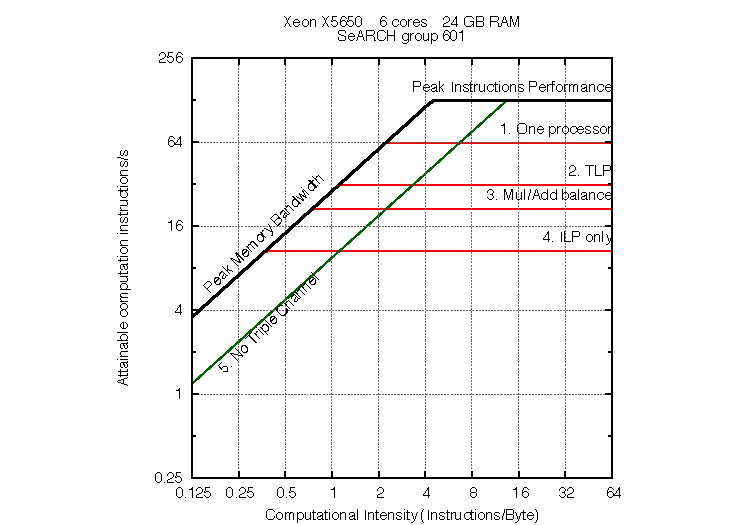
\includegraphics[scale=0.9]{../../common/601.pdf}
		\caption{Roofline models for the compute-601 system used in the \ttDilepKinFit computational characterization.}
		\label{fig:Roofline601}
	\end{center}
\end{figure}

